\documentclass[11pt,a4paper]{article}

\usepackage[utf8]{inputenc}
\usepackage[T1]{fontenc}
\usepackage[margin=1in]{geometry}
\usepackage{amsmath,amssymb,amsfonts}
\usepackage{graphicx}
\usepackage{xcolor}
\usepackage{booktabs}
\usepackage{tabularx}
\usepackage{array}
\usepackage{listings}
\usepackage{tikz}
\usetikzlibrary{shapes.geometric, arrows.meta, positioning, calc, fit}
\usepackage{enumitem}
\usepackage{caption}
\usepackage{subcaption}
\usepackage{float}
\usepackage{hyperref}

\hypersetup{
    colorlinks=true,
    linkcolor=black,
    citecolor=black,
    urlcolor=blue!70!black,
    pdftitle={FTP Server and Client},
    pdfauthor={Subham Bhat}
}

\definecolor{codebg}{rgb}{0.96,0.96,0.96}
\definecolor{codeframe}{rgb}{0.25,0.25,0.25}
\definecolor{codenum}{rgb}{0.45,0.45,0.45}

\lstset{
    backgroundcolor=\color{codebg},
    basicstyle=\ttfamily\footnotesize,
    breakatwhitespace=false,
    breaklines=true,
    captionpos=b,
    commentstyle=\color{codenum}\itshape,
    keywordstyle=\bfseries,
    numberstyle=\tiny\color{codenum},
    numbers=left,
    numbersep=8pt,
    frame=single,
    rulecolor=\color{codeframe},
    tabsize=4,
    columns=flexible,
    keepspaces=true,
    showspaces=false,
    showstringspaces=false,
    xleftmargin=14pt,
    xrightmargin=4pt,
    literate={→}{{$\rightarrow$}}1 {←}{{$\leftarrow$}}1 {–}{{--}}1 {—}{{---}}1 {·}{{$\cdot$}}1 {✓}{{OK}}2 {✗}{{X}}1
}

\newcolumntype{Y}{>{\raggedright\arraybackslash}X}

% screenshot from docs/screenshots (skipped quietly if the file is missing)
\newcommand{\shot}[3][0.92\textwidth]{%
  \IfFileExists{docs/screenshots/#2}{%
  \begin{figure}[H]\centering
  \includegraphics[width=#1,keepaspectratio]{docs/screenshots/#2}
  \caption{#3}\end{figure}}{}}

\emergencystretch=3em
\setlength{\parindent}{1.5em}
\setlength{\parskip}{0.4em}

\begin{document}

% ==============================================================================
% TITLE PAGE
% ==============================================================================
\begin{titlepage}
    \centering
    \vspace*{4.2cm}

    {\LARGE \textbf{File Transfer Protocol: Two Connections,}}\\[0.7em]
    {\LARGE \textbf{Active vs Passive Mode, ASCII vs Binary,}}\\[0.7em]
    {\LARGE \textbf{Resume, FTPS, and Bounce Protection}}\\[1.4em]

    {\large for Computer Networks Laboratory}

    \vspace{3.8cm}

    {\large
    \textbf{Name:} Subham Bhat\\[0.55em]
    \textbf{Class:} BCSE III\\[0.55em]
    \textbf{Roll:} 002410501020\\[0.55em]
    \textbf{Group:} A1\\[0.55em]
    \textbf{College:} Jadavpur University
    }

    \vfill
    {\normalsize 1}
\end{titlepage}

% ==============================================================================
% TABLE OF CONTENTS
% ==============================================================================
\pagenumbering{roman}
\setcounter{page}{2}
\tableofcontents
\newpage

% ==============================================================================
% MAIN CONTENT
% ==============================================================================
\pagenumbering{arabic}
\setcounter{page}{3}

\section{Introduction}
\noindent The \textbf{File Transfer Protocol} (\textbf{FTP}, \textbf{RFC 959}) copies files between a client and a server. It is older than the web and has one design decision that makes it unique among the common application protocols: it uses \textbf{two TCP connections}.
\begin{itemize}[leftmargin=2em]
    \item The \textbf{control connection} (server port 21) stays open for the whole session and carries text commands (\texttt{USER}, \texttt{RETR}, \ldots) and three-digit replies. This is called \emph{out-of-band} control.
    \item A separate \textbf{data connection} is opened for every file transfer or directory listing and closed at its end; the close marks the end of the file.
\end{itemize}
Who opens the data connection depends on the mode. In \textbf{active mode} (\texttt{PORT}) the \emph{server} connects back to a port the client announced, which client-side firewalls and NAT routers block. In \textbf{passive mode} (\texttt{PASV}) the \emph{client} connects to a port the server opened, which is why every modern client defaults to it. FTP also distinguishes \textbf{ASCII} (\texttt{TYPE A}) transfers, which convert line endings, from \textbf{binary} (\texttt{TYPE I}) transfers, which copy bytes exactly. Like Telnet, plain FTP sends the password in clear text; \textbf{FTPS} (RFC 4217) adds TLS.

\subsection{What Was Built}
This module implements an FTP server and client from the RFCs in pure Java 11 with no external libraries:
\begin{enumerate}[leftmargin=2em]
    \item \textbf{Server}: RFC 959 commands, active mode with \texttt{PORT}/\texttt{EPRT} (the server connects from port 20-style \emph{control port $-$ 1}), passive mode with \texttt{PASV}/\texttt{EPSV} (RFC 2428), \texttt{TYPE A} and \texttt{TYPE I}, \texttt{REST} and \texttt{ABOR}, \texttt{SIZE}, \texttt{MDTM} and \texttt{FEAT} (RFC 3659), a per-user home directory jail, anonymous read-only access, and \textbf{FTPS} with \texttt{AUTH TLS}, \texttt{PBSZ} and \texttt{PROT P}.
    \item \textbf{Security}: \textbf{bounce-attack protection} (RFC 2577) and salted SHA-256 password hashes.
    \item \textbf{Client}: the same modes, with an optional simulated client firewall that blocks incoming connections.
    \item \textbf{Wire tap} on the control connection, showing the password in plain FTP and only TLS records in FTPS.
    \item \textbf{Dashboard} on \texttt{http://localhost:8086} that draws the two connections as a signal wire (control) and a track (data) and steps through every command and reply.
\end{enumerate}

\begin{table}[H]
\centering
\caption{Ports and accounts}
\small
\begin{tabularx}{\textwidth}{@{}lY@{}}
\toprule
\textbf{Item} & \textbf{Value} \\ \midrule
Control connection & TCP 2121 (also the real port 21 when it is free) \\
Active-mode data & from TCP 2120 (control port $-$ 1, the analogue of port 20) \\
Passive-mode data & TCP 50000--50100 \\
Wire tap & TCP 2122 $\rightarrow$ 2121 \\
Dashboard & HTTP 8086 \\
Users & \texttt{alice/alice123}, \texttt{bob/bob123}, \texttt{subham/ju2026}, \texttt{anonymous} (read-only) \\ \bottomrule
\end{tabularx}
\end{table}

\shot{01_file_transfer_protocol.png}{The FTP dashboard.}

% ==============================================================================
\section{Commands and Replies}
Commands are ASCII lines ending in \texttt{CRLF}. Every reply begins with three digits; the first gives the outcome and the second the subject.

\begin{table}[H]
\centering
\caption{Meaning of the reply-code digits}
\small
\begin{tabularx}{\textwidth}{@{}clcl@{}}
\toprule
\textbf{1st} & \textbf{Outcome} & \textbf{2nd} & \textbf{Subject} \\ \midrule
1 & Preliminary: started, wait for another reply & 0 & Syntax \\
2 & Completed & 1 & Information \\
3 & Intermediate: send the next command & 2 & Connections \\
4 & Transient failure: try again later & 3 & Authentication \\
5 & Permanent failure & 5 & File system \\ \bottomrule
\end{tabularx}
\end{table}

\begin{lstlisting}[numbers=none, caption={A passive-mode download, as recorded by the dashboard (C = client, S = server).}]
   TCP connection 57026 -> 127.0.0.1:2121        the CONTROL connection, kept for the whole session
S: 220 JU-FTP ready . RFC 959 . ftp.cse.myuniv.edu
C: USER alice
S: 331 Password required for alice
C: PASS ********                                  travels in PLAINTEXT unless AUTH TLS came first
S: 230 User alice logged in, home /home/alice
C: TYPE I
S: 200 TYPE set to I (binary: bytes sent exactly as stored)
C: PASV
S: 227 Entering Passive Mode (127,0,0,1,195,80)   port = 195 x 256 + 80 = 50000
   DATA connection: client 57027 -> server 50000 (the client opens it)
C: RETR /pub/rfc959-notes.txt
S: 150 Opening BINARY mode data connection for /pub/rfc959-notes.txt (231 bytes)
   DATA connection closed . 231 bytes             end of file = end of the data connection
S: 226 Transfer complete: 231 bytes in 5 ms
C: QUIT
S: 221 Goodbye
\end{lstlisting}

% ==============================================================================
\section{System Architecture}

\begin{figure}[H]
\centering
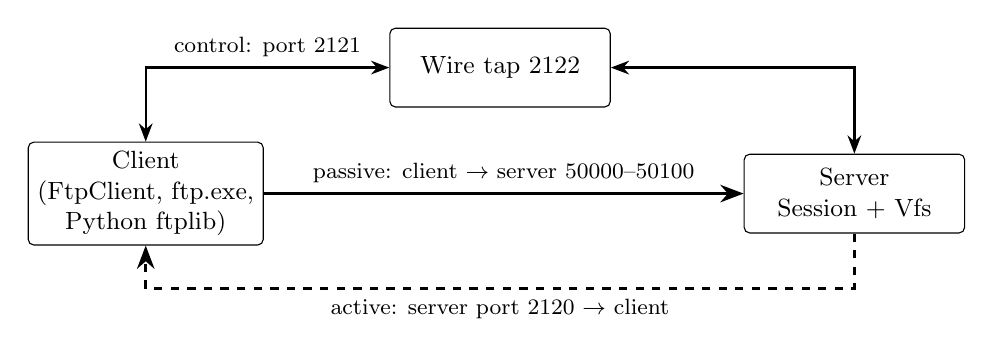
\begin{tikzpicture}[box/.style={draw, rounded corners=2pt, minimum width=2.8cm, minimum height=1.0cm, align=center, font=\small}, >=Stealth]
\node[box] (c) at (0,0) {Client\\(FtpClient, ftp.exe,\\Python ftplib)};
\node[box] (s) at (9,0) {Server\\Session + Vfs};
\node[box] (t) at (4.5,1.6) {Wire tap 2122};
\draw[<->, thick] (c.north) |- node[above, pos=0.75, font=\footnotesize]{control: port 2121} (t.west);
\draw[<->, thick] (t.east) -| (s.north);
\draw[->, very thick, dashed] (s.south) -- ++(0,-0.7) -| node[below, pos=0.25, font=\footnotesize]{active: server port 2120 $\rightarrow$ client} (c.south);
\draw[->, very thick] (c.east) -- node[above, font=\footnotesize]{passive: client $\rightarrow$ server 50000--50100} (s.west);
\end{tikzpicture}
\caption{One control connection, and a new data connection per transfer opened by either side.}
\end{figure}

\begin{table}[H]
\centering
\caption{Source files}
\small
\begin{tabularx}{\textwidth}{@{}lY@{}}
\toprule
\textbf{File} & \textbf{Responsibility} \\ \midrule
\texttt{server/FtpServer.java} & Listener, users and hashes, passive port range, settings (anonymous, slow link). \\
\texttt{server/Session.java} & One control connection: command dispatch, data connections, transfers, TLS. \\
\texttt{server/Vfs.java} & Virtual file system with a home-directory jail per user. \\
\texttt{server/Codes.java} & Reply-code meanings and the ASCII line-ending conversion. \\
\texttt{client/FtpClient.java} & Client with active/passive mode, firewall simulation and FTPS. \\
\texttt{tap/Tap.java} & Control-connection sniffer. \\
\texttt{dashboard/DashboardServer.java} & HTTP API and step-by-step traces. \\ \bottomrule
\end{tabularx}
\end{table}

% ==============================================================================
\section{Implementation}

\subsection{Active and Passive Data Connections}
For \texttt{PORT h1,h2,h3,h4,p1,p2} the server records the client's address and port ($p_1 \times 256 + p_2$) and connects there at the next transfer, binding its own end to \emph{control port $-$ 1}. For \texttt{PASV} it opens a listening socket from its passive range and announces it in the same six-number format; \texttt{EPSV} announces only the port (\texttt{229 (|||port|)}), which also works for IPv6.

\textbf{Bounce-attack protection.} RFC 959 allows \texttt{PORT} to name \emph{any} host, so an attacker could make the server open connections to a third machine on its behalf (the FTP bounce attack, RFC 2577). The server only connects back to the address of the control connection and never to a privileged port.

\begin{lstlisting}[language=Java, caption={PORT, PASV and bounce protection in \texttt{server/Session.java}.}]
private void port(String a) {
    String[] p = a.split(",");
    if (p.length != 6) { reply("501 PORT h1,h2,h3,h4,p1,p2"); return; }
    activeTo(p[0] + "." + p[1] + "." + p[2] + "." + p[3],
             Integer.parseInt(p[4].trim()) * 256 + Integer.parseInt(p[5].trim()), "PORT");
}
private void activeTo(String ip, int port, String how) {
    // RFC 2577: only connect back to the client itself, never to a privileged port
    if (!ip.equals(ctrl.getInetAddress().getHostAddress()) || port < 1024) {
        reply("500 Illegal " + how + " command: " + ip + ":" + port + " (bounce-attack protection, RFC 2577)");
        return;
    }
    closePasv();
    active = new InetSocketAddress(ip, port);
    reply("200 " + how + " ok: I will connect to " + ip + ":" + port + " for the next transfer (active mode)");
}
private void pasv(boolean extended) throws IOException {
    closePasv(); active = null;
    pasv = srv.pasvSocket(ctrl.getLocalAddress());           // a port from 50000-50100
    int p = pasv.getLocalPort();
    byte[] a = ctrl.getLocalAddress().getAddress();
    if (extended) reply("229 Entering Extended Passive Mode (|||" + p + "|)");
    else reply(String.format("227 Entering Passive Mode (%d,%d,%d,%d,%d,%d)",
            a[0] & 0xFF, a[1] & 0xFF, a[2] & 0xFF, a[3] & 0xFF, p / 256, p % 256));
}
\end{lstlisting}

\begin{lstlisting}[language=Java, caption={Opening the data connection: accept in passive mode, connect from port control$-$1 in active mode.}]
private Socket openData() throws IOException {
    Socket s;
    if (pasv != null) {
        pasv.setSoTimeout(10_000);
        try { s = pasv.accept(); } finally { closePasv(); }      // passive: the CLIENT connects
    } else if (active != null) {
        InetSocketAddress to = active; active = null;
        s = new Socket(); s.setReuseAddress(true);
        int src = ctrl.getLocalPort() - 1;                       // like port 20 next to port 21
        try { s.bind(new InetSocketAddress(ctrl.getLocalAddress(), src)); }
        catch (BindException e) { s.close(); s = new Socket(); }
        s.connect(to, 4000);                                     // active: the SERVER connects
    }   // (a transfer without PORT or PASV is refused earlier with "425 Use PORT or PASV first")
    return s;
}
\end{lstlisting}

\subsection{ASCII vs Binary}
In ASCII mode the data is sent as NVT-ASCII: every line ends in \texttt{CRLF} on the wire, whatever the local convention. A Unix text file therefore grows by one byte per line. Applied to an image, the same conversion inserts a \texttt{0D} before every \texttt{0A} byte and corrupts it.

\begin{lstlisting}[language=Java, caption={ASCII mode on the wire (\texttt{server/Codes.java}).}]
/** ASCII mode on the wire: every LF becomes CRLF (RFC 959 NVT-ASCII). */
public static byte[] toCrlf(byte[] d) {
    ByteArrayOutputStream b = new ByteArrayOutputStream(d.length + d.length / 16);
    int prev = -1;
    for (byte x : d) { int c = x & 0xFF; if (c == '\n' && prev != '\r') b.write('\r'); b.write(c); prev = c; }
    return b.toByteArray();
}
\end{lstlisting}

\subsection{Abort and Resume}
\texttt{ABOR} on the control connection stops a transfer in progress: the server closes the data connection and replies \texttt{426} (transfer aborted) followed by \texttt{226} (abort successful). \texttt{REST n} before \texttt{RETR} makes the server skip the first $n$ bytes, so an interrupted download continues where it stopped; the dashboard verifies that the resumed file is byte-identical to the original. HTTP's \texttt{Range} header solves the same problem in the HTTP module.

\subsection{Security: Jail, Anonymous Access and FTPS}
Each user is confined to a home directory: \texttt{CWD ../../..} stays at \texttt{/}, and \texttt{MKD} outside the home directory returns \texttt{550}. Anonymous users see only \texttt{/pub} and cannot store files (\texttt{553}). For FTPS the client sends \texttt{AUTH TLS}; after \texttt{234} both ends perform a TLS handshake on the control connection, then \texttt{PBSZ 0} and \texttt{PROT P} extend protection to the data connections. The wire tap shows \texttt{PASS alice123} on a plain session and only TLS records after \texttt{AUTH TLS}.

% ==============================================================================
\section{Experiments, Verification and Results}

\subsection{Running the Module}
\begin{lstlisting}[language=bash, caption={Starting the server, running the checks, and using real clients.}]
cd FTP
run.bat                  # server, wire tap and dashboard (http://localhost:8086)
run.bat --verify         # 32 automated checks
python interop_test.py   # Python ftplib (plain + FTPS) and Windows ftp.exe (10 checks)

ftp 127.0.0.1            # Windows ftp.exe uses active mode: user alice, then binary, get /pub/logo.png
\end{lstlisting}

\subsection{Active vs Passive Behind a Firewall}
The dashboard runs \texttt{LIST /pub} in both modes side by side, with and without a simulated client firewall that drops incoming connections.

\begin{table}[H]
\centering
\caption{Observed results}
\small
\begin{tabularx}{\textwidth}{@{}lYY@{}}
\toprule
 & \textbf{Active (PORT)} & \textbf{Passive (PASV)} \\ \midrule
No firewall & \texttt{200 PORT ok}; the server connects from port 2120 to the client; \texttt{226}, listing received & \texttt{227}; the client connects to port 5000x; \texttt{226}, listing received \\
Client firewall & The server's incoming connection is dropped: \textbf{\texttt{425 Can't open data connection}} & The client's outgoing connection passes: listing received \\ \bottomrule
\end{tabularx}
\end{table}

\shot{02_two_connections.png}{The two connections drawn as a signal wire (control) and a track (data).}

\subsection{Automated Verification}
All \textbf{32 checks} of \texttt{Verify.java} and all \textbf{10} interoperation checks pass.

\begin{table}[H]
\centering
\caption{Selected verification checks (all passed)}
\small
\begin{tabularx}{\textwidth}{@{}Y@{}}
\toprule
220 greeting; \texttt{USER} $\rightarrow$ 331; wrong \texttt{PASS} $\rightarrow$ 530; right \texttt{PASS} $\rightarrow$ 230 \\
\texttt{FEAT}: multi-line 211 reply lists SIZE, REST, EPSV, AUTH TLS; unknown command $\rightarrow$ 502 \\
\texttt{CWD ../../..} cannot escape the jail; \texttt{MKD} outside the home folder $\rightarrow$ 550 \\
Passive LIST (client connects); active LIST (server connects from port control$-$1) \\
Active behind a client firewall $\rightarrow$ 425; passive behind the same firewall still works \\
\texttt{EPSV} $\rightarrow$ 229 (|||port|); \texttt{PORT} to another host $\rightarrow$ 500 (bounce-attack protection) \\
\texttt{RETR} and \texttt{STOR} in binary: byte-identical image; the same image uploaded in ASCII mode is corrupted \\
ASCII \texttt{RETR} of a text file: every LF becomes CR LF on the wire \\
\texttt{SIZE} and \texttt{MDTM} $\rightarrow$ 213; \texttt{RNFR}/\texttt{RNTO}/\texttt{DELE} \\
\texttt{ABOR} half-way: 426 then 226; \texttt{REST} resumes and the file is byte-identical \\
Anonymous login sees \texttt{/pub}; anonymous \texttt{STOR} $\rightarrow$ 553 \\
FTPS: \texttt{AUTH TLS} + \texttt{PBSZ 0} + \texttt{PROT P}, then an encrypted \texttt{RETR} \\
The wire tap reads the password on plain FTP and sees only TLS records after \texttt{AUTH TLS} \\ \bottomrule
\end{tabularx}
\end{table}

\subsection{Observations}
\begin{enumerate}[leftmargin=2em]
    \item \textbf{Two connections make the firewall problem.} Active mode failed with 425 as soon as the client refused incoming connections, while passive mode worked; this is the practical reason for passive mode and EPSV.
    \item \textbf{Transfer type matters.} The ASCII-mode copy of a PNG was rejected by the image decoder, while the binary copy had the same SHA-256 hash as the original.
    \item \textbf{Standard clients work.} Python's \texttt{ftplib} (plain and FTPS) and Windows \texttt{ftp.exe} (which uses active mode) completed logins, listings and transfers against the server.
\end{enumerate}

% ==============================================================================
\section{Conclusion}
\begin{enumerate}[leftmargin=2em]
    \item \textbf{Out-of-band control is FTP's defining feature.} Keeping commands on one long-lived connection and data on short per-transfer connections makes aborting and resuming simple, but it doubles the number of connections a firewall must allow.
    \item \textbf{Passive mode exists because of firewalls and NAT.} The experiment reproduced the 425 failure of active mode behind a client firewall and showed passive mode succeeding.
    \item \textbf{FTP needs both protection and encryption.} Restricting \texttt{PORT} to the client's own address blocks the bounce attack, the jail confines users, and \texttt{AUTH TLS} removes the plaintext password that the wire tap otherwise recovers.
\end{enumerate}

\section*{AI Acknowledgement}
\addcontentsline{toc}{section}{AI Acknowledgement}
Artificial Intelligence tools were used as an aid during this project. Specifically, AI assistance was used for:
\begin{itemize}[leftmargin=2em]
    \item \textbf{Protocol cross-checking:} comparing message formats, reply codes, state machines and byte offsets against the RFCs cited in this report.
    \item \textbf{Code review and testing:} suggesting edge cases for the automated verification suite and reviewing concurrency and error handling.
    \item \textbf{Writing and visualization:} drafting, structuring and refining the explanations, tables, diagrams and \LaTeX{} source of this report.
\end{itemize}
All protocol implementations, Java source code, experiments, measurements and final conclusions were run, reviewed and verified by the author, who takes full responsibility for the content of this report.

\end{document}
